\section{Lecture 2}
Supervised learning of behaviors and imitation learning
\subsection{Part 1}
\subsubsection{Notation and Context}
Given an observation $o$, our goal is to find a policy $\pi_\theta(a_t|o_t)$ that maps an observation to an action at a time $t$.
\begin{itemize}
    \item $\textbf{o}_t$ - observation
    \item $\textbf{s}_t$ - state (note that this and observation tend to get confounded)
    \item $\textbf{a}_t$ - action
    \item $\pi_\theta(\textbf{a}_t|\textbf{o}_t)$ - policy which can be deterministic or stochastic. We can generalize policies to be stochastic and then if we want a deterministic decision we can pick the most probable outcome.
    \item $\pi_\theta(\textbf{a}_t|\textbf{s}_t)$ - policy (fully observed)    
\end{itemize}

\begin{figure}[htbp]
  \centerline{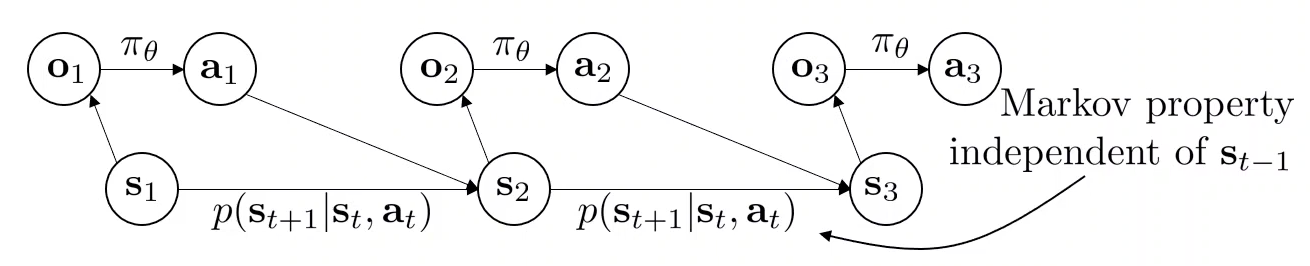
\includegraphics[width=0.75\textwidth]{images/lecture2_grapical_depiction}}
  \caption{Graphical model showing the transition of observations, actions, and states}
  \label{fig:lecture2_grapical_depiction}
\end{figure}

\subsubsection{Imitation Learning}
Imitation learning's goal is to get a policy from looking at observations and actions. Observation and action pairs $(\textbf{o}_t,\textbf{a}_t)$ are taken in as training data and fed into some supervised learning algorithm with the goal of outputting a policy $\pi_\theta(\textbf{a}_t | \textbf{o}_t )$. Imitation learning, or behavior cloning, can be very flawed since it is difficult for it to adapt its knowledge to new situations. The supervised learning model will make a mistake that gets compounded as mistakes will cause it to deviate from the original trajectory. Being in a new trajectory increases the likelihood that the model will make more mistakes.
\\ 
The issue of compounded mistakes is not present in traditional supervised learning since each observation in the data is IID. In a temporal sequence, like a control/reinforcement learning problem, the IID assumption does not hold. This issue can be avoided or mitigated by being smart about the way data is collected and augmented.

\subsection{Part 2}
\subsubsection{Why does behavioral cloning fail?}
If we have a policy $\pi_\theta( \textbf{a}_t | \textbf{o}_t)$ and a data set $(\textbf{o}_t, \textbf{a}_t)$. We can define the probabilities that we pick an action based off of an observation as $p_{data}(\textbf{o}_t)$ and $p_{\pi_\theta} (\textbf{o}_t)$. In this case, as we train using supervised learning, we have the objective function 
\begin{equation}
     \max_\theta \mathbb{E}_{\textbf{o}_t ~ p_{data}(\textbf{o}_t)} [\log \pi_\theta(\textbf{a}_t | \textbf{o}_t)]
\end{equation}
Since there is a difference in the distribution that the model was trained on and the one that it will experience $p_{data}(\textbf{o}_t)$ and $p_{\pi_\theta} (\textbf{o}_t)$, this skews the output. A different objective function can be created using a cost function
\begin{equation}
    c(\textbf{s}_t, \textbf{a}_t) = 
    \begin{cases}
        0 \quad if \textbf{a}_t = \pi^*(\textbf{s}_t)\\ 
        1 \quad otherwise
    \end{cases}
\end{equation}
and we restructure our objective function to be
\begin{align}
  \text{minimize} & \quad \mathbb{E}_{\textbf{s}_t ~ p_{\pi_\theta}(\textbf{s}_t)} [c(\textbf{s}_t, \textbf{a}_t)]
\end{align}
We can analyze how effective behavioral cloning by identifying how likely you are at each time step $t$ in a horizon $T$ to make a mistake. If we assume that for any $\textbf{s} \in D_{train}$, there is a probability $\textbf{prob} [\pi_\theta(\textbf{a} \neq \pi^* (\textbf{s}) | \textbf{s})] \leq \epsilon$. Then if we want to find the expected value of our cost function across all time periods, we can find the below equation. Intuitively, the below equation works by first adding the probability we make a mistake each period to the probability we don't make a mistake on the first step and then every mistake every step after, etc.

\begin{equation}
    \mathbb{E}[\sum_{t} c(\textbf{s}_t, \textbf{a}_t)] \leq \epsilon T + (1-\epsilon)(\epsilon(T-1)) \dots 
\end{equation}

This series increases at a rate $O(\epsilon T^2)$ in the worst case. This is a pessimistic worst case, so in order for behavioral cloning to work in practice, the cost functions and problem structure is usually built in a way to make the state easy to recover from.